
\section{Atomic orbital basis}

\noindent ii) \uline{Atomic orbital basis (lattice fermions)}

\noindent We now consider a system where fermions most of the time stay localized on sites on a lattice. Occasionally, they may tunnel from one lattice site to another. This tunneling arises because the long-distance (away from lattice sites) tails of the atomic orbitals (Wannier-functions) may overlap.

\begin{center}
	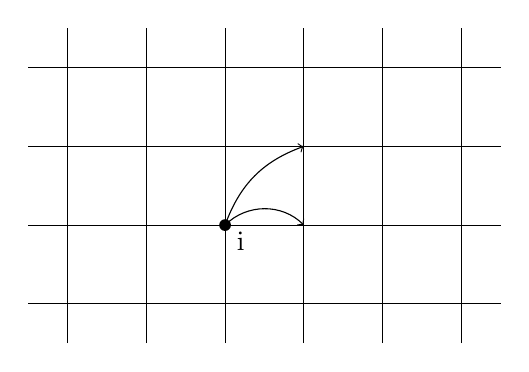
\begin{tikzpicture}
		\draw[step=1.0,black,thin] (0.5,0.5) grid (6.5,4.5);	
		\draw[->] (3,2)  to [out=70,in=200, looseness=1] (4,3);
		\draw[->] (3,2)  to [out=45,in=135, looseness=1] (4,2);
		\node at (3,2) [circle,fill,inner sep=1.5pt]{};
		\node at (3.2,1.8) {i};
	\end{tikzpicture}
\end{center}
\noindent Two tunneling processes ("hopping") on a 2D rectangular lattice, from lattice site \uline{i} to its \uline{nearest} and \uline{next-nearest} neighbors. The long distance tails of the Wannier-functions fall off exponentially (recall the wave-functions of the Hydrogen-atom). Therefore, hopping is most likely to occur from a lattice site i to its nearest neighbor. The next most probable hopping event is a direct hopping from i to its next-nearest neighbor, or two hopping via an intermediate nearest neighbor. Which process is most likely is a matter of some detail: The two factors that mostly determine this is the distance between atoms on the lattice, and the type of atoms which are situated on the lattice points. If $\Delta \vb{r}$ is the separation between the electron and the ionic position, then the Wannier-functions fall off approximately as $\e^{-\Delta \vb{r}/\lambda}$
\begin{align*}
	\lambda = c \frac{a_0}{Z}
\end{align*}

\noindent $c$: Constant of order unity \newline
\noindent $a_0$: Bohr-radius\newline
\noindent $Z$: Number of protons in the nucleus\newline

\noindent For heavy atoms, Wannier orbitals are more tightly localized around atoms than in lighter elements. \newline
Crystal potential (rigid crystal) \newline

\noindent $U= \sum_i U(\vb{r}_i) $ \\
\noindent $U(\vb{r}_i)= \sum_j U(\vb{r}_i, \vb{R}j)$\\
\noindent $\vb{r}_i$: Electronic coordinate ; $\vb{R}j$: Ionic coordinate.\\

\noindent $U_a(\vb{r}_i, \vb{R}j)$: Potential energy that electron at $\vb{r}_i$ feels from ion located at $\vb{R}j$. The dominant contribution to this is when $i=j$, i.e. when the electron and ion is on the same site $i$. We single out this contribution as follows
\begin{align*}
	U = \sum_i U_a(\vb{r}_i, \vb{r}_i) + \sum_i \sum_{j\neq i}  U_a(\vb{r}_i, \vb{R}j).
\end{align*}
\noindent The point of this splitting is that the basis functions $\{\varphi_\lambda \}$ that we will choose, will be the eigenfunctions of the total Hamilton-operator for \uline{isolated} atoms. This is a very natural choice for a system where electrons spend most of the time on isolated atoms and only relatively rarely hop from one site to the other.\newline

\noindent Schrödinger-equation for isolated atoms:

\begin{align*}
	\left[\frac{\vb{p}_i^2}{2m}+ U_a( \vb{r}_i, \vb{R}_i)\right] \varphi_{\alpha, \sigma}( \vb{r}_i, s_i)= \varepsilon_{\alpha,\sigma, i} \varphi_{\alpha, \sigma}( \vb{r}_i, s_i)
\end{align*}

\noindent $\alpha$: Index for atomic orbital \\
\noindent $\sigma$: Spin quantum number\\
\noindent $\vb{r}_i$: Spatial coordinate of electron on lattice site $i$\\
\noindent $\sigma_i$: Spin-coordinate of electron on lattice site $i$r\\
\noindent $\varepsilon_{\alpha,\sigma, i}$: Energy of electron in orbital $\alpha$ on lattice site$i$. In principle this energy could vary from lattice site to lattice site, but for most systems we will let $\varepsilon_{\alpha, \sigma, i} = \varepsilon_{\alpha, \sigma}$ i.e. independent of the position on the lattice. In principle, $\varepsilon_{\alpha, \sigma}$ could depend on spin. 
If we now bring in the rest of the crystal potential (from the surrounding atoms) in the one-particle Hamiltonian, the basis set $\{\varphi_\lambda \}$ that we have chosen, are no longer eigenfunctions of the Hamiltonian. This leads to scattering from one state $\ket{\lambda}$ to another state $\ket{\lambda'}$, and this in term gives rise to tunneling, or hopping, of electrons on the lattice. Thus, the hopping of electrons around on the lattice, which represents kinetic energy, originates with the crystal potential from surrounding atoms working on an electron. The details are as follows:

\begin{align*}
	&\varphi_{\alpha, \sigma,j}(\vb{r}_i,s_i) = \Phi_{\alpha, j}^W (\vb{r}_i) \cdot \chi_\sigma (s_i)\\
	&\lambda = (\alpha, \sigma, j)
\end{align*}
(\uline{Note}: $\alpha$ must be thought of as consisting of two numbers: (l,m) of a hydrogen-like atom.)\\

\noindent Field operator:
\begin{align*}
	\psi^\dagger_j(\vb{r}_i, s_i, t)= \sum_{\alpha, \sigma} \cd_{\alpha, \sigma, i} \Phi_{\alpha, j}^* (\vb{r}_i) \cdot \chi^*_\sigma (s_i)
\end{align*}
\begin{align*}
	\{ c_{\alpha, \sigma, i},\cd_{\alpha', \sigma', i'} \} = \delta_{\alpha, \alpha'} \delta_{\sigma,\sigma'} \delta_{i,i'}
\end{align*}
Other commutators are zero.\\

\noindent \uline{Orthogonality}:

\begin{align*}
	\sum_{\vb{r}} \sum_s  \varphi^*_{\alpha, \sigma,j}(\vb{r},s)\varphi_{\alpha', \sigma',j'}(\vb{r},s) \cong \delta_{\alpha, \alpha'} \delta_{\sigma,\sigma'} \delta_{j,j'}
\end{align*}

\noindent \uline{Completeness}:

\begin{align*}
	\sum_{\alpha, \sigma, j} \varphi^*_{\alpha, \sigma,j}(\vb{r},s)\varphi_{\alpha, \sigma,j}(\vb{r}',s') \cong \delta_{\vb{r},\vb{r}'} \delta_{s,s'} 
\end{align*}

\subsection{Single particle Hamiltonian}
\suggestion{Forslag for del-overskrift.}
\begin{align*}
	\Ha_1 = \sum_i \left( \frac{\vb{p}_i^2}{2m}+ U_a (\vb{r}_i, \vb{R}_i) \right) + \sum_i \sum_{j \neq i} U_a ( \vb{r}_i, \vb{R}_j)
\end{align*}

\noindent Since the basis-functions are assumed to be eigenfunctions of the first term, we have:

\begin{equation}
	\sum_i  \frac{\vb{p}_i^2}{2m}+ U_a (\vb{r}_i, \vb{R}_i)\implies  \sum_{\alpha, \sigma, i} \varepsilon_{\alpha, \sigma, i} \cd_{\alpha, \sigma, i} c_{\alpha, \sigma, i}
\end{equation}

\noindent Consider now the term

\begin{align*}
	& \sum_i \sum_{j \neq i} U_a ( \vb{r}_i, \vb{R}_j)\\
	\implies & H_{12} = \sum_{{\lambda_{1}}, {\lambda_{2}}} \bra{\lambda_{1}}  \sum_{j \neq i} U_a ( \vb{r}_i, \vb{R}_j) \ket{\lambda_{2}} \cd_{ \lambda_1} c_{\lambda_{2}}\\
	&= \sum_{\alpha_1, \sigma_1, i_1} \sum_{\alpha_2, \sigma_2, i_2} \bra{\alpha_1, \sigma_1, i_1} \sum_{j \neq i_2} U_a \ket{\alpha_2, \sigma_2, i_2} \cd_{\alpha_1, \sigma_1, i_1} c_{\alpha_2, \sigma_2, i_2}
\end{align*}

The matrix element: 

\begin{align*}
	&\bra{\alpha_1, \sigma_1, i_1} \sum_{j \neq i_2} U_a \ket{\alpha_2, \sigma_2, i_2}\\
	&= \sum_s \sum_{\vb{r}} \varphi_{\alpha_1, \sigma_1, i_1}^* (\vb{r},s) \underbrace{\left[\sum_{j\ne i_2} U_a (\vb{r},\vb{R}_j) \right] }_{\mathclap{\text{Sum from surrounding atoms}}}  \varphi_{\alpha_2, \sigma_2, i_2}(\vb{r},s)
\end{align*}

Here, we have used
\begin{equation}
	\mel{\vb{r},s}{U_a(\vb{r},\vb{R}_j)}{\vb{r}',s'}= U_a(\vb{r},\vb{R}_j)\delta_{\vb{r},\vb{r}'}\delta_{ss'}.
\end{equation}
This may be simplified further, using the fact that $U_a(\vb{r},\vb{R}_j)$ is purely electrostatic and spin-independent.
We use the fact that set $\{\p_{\alpha, \sigma,i}(\vb{r},s)\}$ factorize into a spatial part and a spin-part.
Denoting the spin-independent quantity
\begin{equation}
	\sum_j U_a(\vb{r},\vb{R}_j) \equiv A(\vb{r}),
\end{equation}
The matrix element is
\begin{equation}
	\sum_{\vb{r}}\sum_s \Phi_{\alpha_1, i_1}^{W*} (\vb{r}) A(\vb{r})\Phi_{\alpha_2, i_2}^W(\vb r) \cdot \chi_{\sigma_1}^* (s)\chi_{\sigma_2} (s).
\end{equation}
Summing over $s$ and using orthogonality of the $\chi$'s, we obtain
\begin{equation}
	\mel{\alpha_1,\sigma_1,i_1}{A(\vb{r}_i)}{\alpha_2,\sigma_2,i_2} = \delta_{\sigma_1\sigma_2}\sum_{\vb r}\Phi_{\alpha_1, i_1}^{W*}(\vb r)A(\vb r)\Phi_{\alpha_2, i_2}^{W}(\vb r)
\end{equation}
\todo{Index $i$ i $A(\vb{r}_i)$.}
Spin is conserved during the hopping process.
The remaining spatial integration may be computed, since the crystal potential is assumed to be known, and so are the required Wannier-functions.
We define the following matrix-elements:
\begin{equation}
	t_{\alpha_1,i_1}^{\alpha_2,i_2} \equiv \sum_{\vb r}\Phi_{\alpha_1, i_1}^{W*}(\vb r)A(\vb r)\Phi_{\alpha_2, i_2}^{W}(\vb r).
\end{equation}
We may now write down the second-quantized version of the single-particle contribution to the Hamiltonian for lattice fermions.
\begin{tcolorbox}
	\begin{align}
		\Ha_1 = \sum_{\alpha\sigma i} \ep_{\alpha\sigma i}\cd_{\alpha\sigma i}c_{\alpha\sigma i} + \sum_{\mathclap{\substack{\alpha_1 i_1 \\ \alpha_2 i_2 \\ \sigma}}} t_{\alpha_1,i_1}^{\alpha_2,i_2}\cd_{\alpha_1\sigma_1 i_1}c_{\alpha_2\sigma_2 i_2}
	\end{align}
\end{tcolorbox}
The first term is simply the energy of electrons on isolated atoms on the lattice. The second term describes spin-conserving hopping of electrons from a state ($\alpha_2, i_2$) to a state ($\alpha_1, i_1$). That is, electron hop from lattice site $i_2$ to $i_1$, and in the process, they may end up in a different atomic orbital $\alpha_1$, than the one they started in ($\alpha_2$).

\begin{center}
	\begin{tikzpicture}
		\node (a) at (0,0) {($\alpha_1, i_1$)};
		\node (b) at (3cm,0) {($\alpha_2, i_2$)};
		\draw[->-=0.5] (b) to [out=150,in=30] node[midway,above] {Spin is conserved} (a);
	\end{tikzpicture}
\end{center}

Before we consider the two-particle contribution to $\Ha_1$, let us simplify the one-particle term.
First, we specialize to the important case where $\ep_{\alpha\sigma i} = \ep_{\alpha\sigma}$ i.e. translationally invariant system. Furthermore, we assume $\ep_{\alpha\sigma}$ to be spin-independent, $\ep_{\alpha\sigma} = \ep_{\alpha}$.
Further simplification is obtained by noting that only the most loosely bound electrons around an atom will be able to ``escape'' the atom and hop to a neighboring site. 
We will focus only on these electrons, which means we will focus on a small subset of orbitals $ \alpha  $, and ignore the orbitals containing tightly bound electrons.

The simplest case is obtained by considering the case where only electrons in one particular orbital (the most loosely bound electrons) can hop from one site to the other. 
Then we may drop the orbital index altogether, and we have
\begin{equation}
	\Ha_1 = \sum_{\sigma,i}\ep \cd_{\sigma,i}c_{\sigma i} + \sum_{\mathclap{\substack{i,j\\ \sigma}}}t_{ij}\cd_{\sigma,i}c_{\sigma,j}.
\end{equation}
We may now set $\ep=0$ (a referecnce energy). Furthermore, 
\begin{equation}
	-t_{ij}\equiv \sum_{\vb r}\Phi_{i}^{W*}(\vb r)A(\vb r)\Phi_{j}^{W}(\vb r).
\end{equation}
$t_{ij}$ can be computed from first-principles, since $A$ and $\Phi^{W}$ are known. However, we will rather consider $t_{ij}$ as a phenomenological parameter that can be fittet to numerical or experimental results. 
Thus, wee finally have
\begin{equation}
	\Ha_1 = -\sum_{i,j,\sigma}t_{ij}\cd_{\sigma i}c_{\sigma_j}.
\end{equation}
Typically, one limits the hopping to nearest and next-nearest neighbor hopping. Note that $t_{ij}$ in principle could be complex.

\subsection{Two-particle Hamiltonian}
\suggestion{Forslag for del-overskrift.}
Next:
\begin{equation}
	\sum_{ij}V_{e-e}(\vb{r}_i - \vb{r}_{j}) \rightarrow \sum_{\mathclap{\lambda_1,\dots, \lambda_{4}}}\mel{\lambda_1\lambda_2}{V_{e-e}}{\lambda_3\lambda_4}\cd_{\lambda_1}\cd_{\lambda_2}c_{\lambda_3}c_{\lambda_4}.
\end{equation}
Here, $\lambda = (i,\sigma)$. No orbital index, since we are only considering one (some) orbital. We therefore need to consider the matrix element
\begin{align*}
	&\mel{i_1\sigma_1\, i_2\sigma_2}{V_{e-e}}{i_3\sigma_3\, i_4\sigma_4} \\[1.5ex]
	&\qquad = \sum_{\mathclap{x_1,\dots,x_4}}\p_{i_1\sigma_1}^*(x_1)\p_{i_2\sigma_2}^*(x_2)V_{e-e}(x_3,x_4)\p_{i_3\sigma_3}(x_3)\p_{i_4\sigma_4}(x_4)\delta_{x_2x_3}\delta_{x_4x_1},
\end{align*}
where $x = (\vb r, s)$.
$V_{e-e}$ is spin-independent, so 
\begin{equation}
	V_{e-e}(x_3, x_4) = V_{e-e}(\vb{r}_3, \vb{r}_4) = V_{e-e}(|\vb{r}_3-\vb{r}_4|).
\end{equation}
Thus, we have, after using the Kronecker-deltas and performing sums over $x_3, x_4$
\begin{align*}
	&\mel{i_1\sigma_1\, i_2\sigma_2}{V_{e-e}}{i_3\sigma_3\, i_4\sigma_4}\\
	&\qquad\qquad = \sum_{\vb{r}_1}\sum_{\vb{r}_2} \Phi_{i_1}^{W*}(\vb r_1)\Phi_{i_2}^{W*}(\vb r_2)V_{e-e}(|\vb{r}_1-\vb{r}_2|)\Phi_{i_3}^{W}(\vb r_2)\Phi_{i_4}^{W}(\vb r_1) \\
	&\qquad\qquad \qquad \cdot \sum_{s_1,s_2}\chi_{\sigma_1}^*(s_1)\chi_{\sigma_2}^*(s_2)\chi_{\sigma_4}(s_1)\chi_{\sigma_3}(s_2)
\end{align*}
Performing the spin-summation:
\begin{equation}
	\sum_{s_1, s_2}\dots \rightarrow \delta_{\sigma_1\sigma_4}\delta_{\sigma_2\sigma_3}.
\end{equation}
Define
\begin{equation}\label{eq:def_Vijkl}
	V_{i_1, i_2, i_3, i_4} \equiv \sum_{\vb{r}_1}\sum_{\vb{r}_2} \Phi_{i_1}^{W*}(\vb r_1)\Phi_{i_2}^{W*}(\vb r_2)V_{e-e}(|\vb{r}_1-\vb{r}_2|)\Phi_{i_3}^{W}(\vb r_2)\Phi_{i_4}^{W}(\vb r_1).
\end{equation}
This quantity expresses the Coulomb-interaction as a \emph{scattering matrix element} of two electrons initially located around lattice sites $(i_3, i_4)$ into two electrons located around lattice sites $(i_1, i_2)$.

Depending on exactly what $(i_3, i_4)$ and $(i_1, i_2)$ are, this scattering element has various physical interpretations. For instance, in the same way that the single particle crystal potential could give rise to single-particle hopping, $V_{e-e}$ may give rise to pair-hopping. Of course, $V_{e-e}$ will also give rise to electrostatic density-density interactions. 

Thus, we have the second-quantized version of the lattice Hamiltonian
\begin{tcolorbox}
	\begin{equation}
		\Ha = -\sum_{i,j,\sigma}t_{ij}\cd_{i\sigma}c_{j\sigma} + \sum_{\mathclap{\substack{i_1,\dots,i_4\\ \sigma_1, \sigma_2}}}V_{i_1,\dots,i_4}\cd_{i_1\sigma_1}\cd_{i_2\sigma_2}c_{i_3\sigma_2}c_{i_4\sigma_1}.
	\end{equation}
\end{tcolorbox}

\subsection{Special cases in scattering matrix}
\suggestion{Forslag for del-overskrift. De står ikke i notatene, men for ryddighets skyld kanskje fornuftig?}
\subsubsection*{All $i$ equal}
Consider next special cases for ($i_1,\dots, i_4$). We expect the largest contribution to $V_{i_1, \dots,i_4}$ when $i_1 = \dots = i_4 (=i)$.
In this case, $\Phi_{i}^{W}(\vb r)$ are all peaked around the same point

\begin{equation}
	V_{iiii} = \sum_{\vb{r}_1}\sum_{\vb{r}_2}|\Phi_{i}^{W}(\vb{r_1})|^2V_{e-e}(|\vb{r}_1-\vb{r}_2|)|\Phi_{i}^{W}(\vb{r}_2)|^2 \equiv U_i.
\end{equation}
Since $ |\Phi_{i}^{W}|^2 $ represents a density, $U$ represents a density-density electrostatic interaction. However, there is a subtle feature pertaining to this interaction, as a result of the fact that we only consider one orbital per site: 
The Hamiltonian reads, considering $i_1 = i_2=i_3=i_4$
\begin{equation}
	\Ha = -\sum_{i,j,\sigma}t_{ij}\cd_{i\sigma}c_{j\sigma} + \sum_{\mathclap{\substack{i\\ \sigma_1, \sigma_2}}}U_i\cd_{i\sigma_1}\cd_{i\sigma_2}c_{i\sigma_2}c_{i\sigma_1}.
\end{equation}
Since the operators ($\cd_{i\sigma},c_{i\sigma}$) create and destroy fermions, we can at most accomodate one fermion per state $\ket{i,\sigma}$. Therefore, in the operator $\cd_{i\sigma_1}\cd_{i\sigma_2}c_{i\sigma_2}c_{i\sigma_3}$\todo{$\sigma_3$ brukes ikke ovenfor?}, we must have
\begin{equation}
	\begin{rcases}
		\sigma_1 =-\sigma_2 \\
		\sigma_2 = -\sigma_3
	\end{rcases}
	\implies \sigma_3 = \sigma_1 = -\sigma_2.
\end{equation}
Thus, upon anti-commuting $c_{i\sigma_3}$ through $c_{i\sigma_2}$ and $\cd_{i\sigma_2}$, we may write this operator as 
\begin{equation}
	\cd_{i,\sigma_1}\cd_{i,-\sigma_1}c_{i,-\sigma_1}c_{i,\sigma_1} = 	\cd_{i,\sigma_1}c_{i,\sigma_1}\cd_{i,-\sigma_1}c_{i,-\sigma_1} = n_{i,\sigma_1}n_{i,-\sigma_1},
\end{equation}
where $n_{i,\sigma_1} = \cd_{i,\sigma_1}c_{i,\sigma_1}$ is a number operator. Thus, the Hamiltonian becomes
\begin{tcolorbox}
	\begin{equation}
		\Ha = - \sum_{i,j,\sigma}t_{ij}\cd_{i\sigma}c_{j\sigma} + \sum_{i,\sigma}U_i n_{i,\sigma}n_{i,-\sigma}.
	\end{equation}
\end{tcolorbox}
This is the so-called \emph{Hubbard-model}, which we may view as an ``Ising-model'' of correlated fermion systems.
In most cases, we consider $U_i = U$ independent of $i$. In that case, it may be solved exactly in one dimension. In two and higher dimensions, no exact solution exists. In fact, very little is known about the properties of this model in more than one dimension, except at a very special point. If we have one fermion pr. site, and $U\gg t_{ij}$, the properties are known, and we will investigate them. When there is more or less than one fermion pr. site on the lattice, the nature of the ground state and the excitations of the model, are not known. 
This model is very important in contemporary condensed matter systems. 
The two-dimensional version is particularily important. It serves as a paradigm model for the physics of high-temperature superconducting copper-oxides, and it also serves, with minor modifications as a model for strongly correlated topological quantum systems, i.e. systems with ground states that have a certain robustness against scattering which is protected by non-trivial topological structure in the space of eigenfunctions. 
The minor modification of the Hubbard model which is required to have it describe correlated topological quantum systems, is to allow the hopping amtrix element $t_{ij}$ to become spin-dependent $t_{ij}\rightarrow t_{ij}^{\sigma\sigma'}$ and complex.
\begin{tcolorbox}
	\begin{equation}
		\Ha = -\sum_{\mathclap{i,j,\sigma,\sigma'}}t_{ij}^{\sigma\sigma'}\cd_{i\sigma}c_{j\sigma'} + U\sum_{i,\sigma}n_{i,\sigma}n_{i,-\sigma}.
	\end{equation}
\end{tcolorbox}
This model is often referred to as the \emph{Kane-Mele-Hubbard model}, here written in a very general form since the complex and spin-dependent $t_{ij}^{\sigma\sigma'}$ is not specified.
Note that so far, there is no reference to precisely \emph{what lattice} this model is defined on.

In the Hubbard-model, we ignore electron-electron two-particle interactions except for when two electrons occupy the same site $ i $ (and if they do, they must have opposite spins). This is clearly a drastic simplification. Nevertheless, the model serves as a useful model if instead of computing $U$ from first principles, we regard it as a phenomenological parameter where screening of the Coulomb potential has been taking into account.
The spin-structure of the density-density interaction $Un_{i\sigma}n_{i-\sigma}$ is interesting. It gives rise to \emph{antiferromagnetism}, as we will see.

\subsubsection*{The case $i_1=i_2, i_3 = i_4$}
\suggestion{Overskrift?}

Consider next the case
\begin{align*}
	\begin{rcases}
		i_1 = i_2 \\
		i_3 = i_4
	\end{rcases} i_1 \ne i_3 &&
	\begin{rcases}
		i_1 \rightarrow i \\
		i_3 \rightarrow j
	\end{rcases} i \ne j.
\end{align*}
We now get a contribution to the two-particle Hamiltonian given by 
\begin{equation}
	\sum_{\mathclap{\substack{i,j \\ \sigma_1, \sigma_2}}}V_{iijj}\cd_{i\sigma_1}\cd_{i\sigma_2}c_{j\sigma_2}c_{j\sigma_1}.
\end{equation}
Again, we see that $\sigma_1 = -\sigma_2$. This term describes a hopping of a two-particle spin-singlet from site $j$ to site $i$.
\begin{center}
	\begin{tikzpicture}
		\node[anchor= north] (a) at (0,0) {\large $(\uparrow\cross\downarrow)_j$};
		\node[anchor=north] (b) at (4cm,0) {\large $(\uparrow\cross\downarrow)_i$};
		\draw[thick,->-=0.5] (a) to [in=150,out=30] (b);
	\end{tikzpicture}
\end{center}
I.e. it is \emph{not} a density-density interaction.

\subsubsection*{The case $i_1=i_4, i_2=i_3$}
Consider next the case 
\begin{align*}
	\begin{rcases}
		i_1 = i_4 \\
		i_2 = i_3
	\end{rcases} i_1 \ne i_2 &&
	\begin{rcases}
		i_1 \rightarrow i \\
		i_2 \rightarrow j
	\end{rcases} i \ne j.
\end{align*}
Contribution to two-particle Hamiltonian is given by
\begin{equation}
	\sum_{\mathclap{\substack{i,j \\ \sigma_1, \sigma_2}}}V_{ijji}\cd_{i\sigma_1}\cd_{j\sigma_2}c_{j\sigma_2}c_{i\sigma_1}.
\end{equation}
Anti-commute $c_{i\sigma_1}$ through $c_{j\sigma_2}$ and $\cd_{j\sigma_2}$ to obtain
\begin{equation}
		\sum_{\mathclap{\substack{i,j \\ \sigma_1, \sigma_2}}}V_{ijji}n_{i\sigma_1}n_{j\sigma_2} = \sum_{i,j}V_{ijji}n_{i}n_{j} \quad ;\quad n_{i} = \sum_{\sigma}n_{i\sigma}.
\end{equation}
This is a purely electrostatic density-density interaction with no spin-structure. (The naive expectation).

\subsubsection*{The case $i_1=i_4, i_2=i_3$}
Consider finally the case
\begin{align*}
	\begin{rcases}
		i_1 = i_3 \\
		i_2 = i_4
	\end{rcases} i_1 \ne i_2 &&
	\begin{rcases}
		i_1 \rightarrow i \\
		i_2 \rightarrow j
	\end{rcases} i \ne j.
\end{align*}
Contribution to the two-particle Hamiltonian given by
\begin{equation}
	\sum_{\mathclap{\substack{i,j \\ \sigma_1, \sigma_2}}}V_{ijij}\cd_{i\sigma_1}\cd_{j\sigma_2}c_{i\sigma_2}c_{j\sigma_1}.
\end{equation}
Anti-commute $c_{i\sigma_2}$ through $\cd_{j\sigma_2}$
\begin{equation}
	-\sum_{\mathclap{\substack{i,j \\ \sigma_1, \sigma_2}}}V_{ijij}\cd_{i\sigma_1}c_{i\sigma_2}\cd_{j\sigma_2}c_{j\sigma_1}.
\end{equation}
There are no restrictions on the values that $\sigma_1$ and $\sigma_2$ can take, and so $\sigma_1$ and $\sigma_2$ may or may not be equal.
When $\sigma_1 = \sigma_2$, the term $\cd_{i\sigma_1}c_{i\sigma_2}$ simply counts the number of particles in spin-state $\sigma_1$ on lattice site $i$. 
If $\sigma_1\ne\sigma_2$, then $\cd_{i\sigma_1}c_{i\sigma_2}$ represents a spin-flip on site $i$.
Let us therefore investigate this a bit further. 

\emph{Consider the operator}
\begin{align*}
	\sum_{\sigma_1, \sigma_2}\cd_{i\sigma_1}c_{i\sigma_2}\cd_{j\sigma_2}c_{j\sigma_1}& \\
	&= \cd_{i\uparrow}c_{i\uparrow}\cd_{j\uparrow}c_{j\uparrow} \qquad \text{(spin up - spin up)} \\
	&+ \cd_{i\uparrow}c_{i\downarrow}\cd_{j\downarrow}c_{j\uparrow} \qquad \text{(flip up - flip down)} \\
	&+\cd_{i\downarrow}c_{i\uparrow}\cd_{j\uparrow}c_{j\downarrow} \qquad \text{(flip down - flip up)}\\
	&+ \cd_{i\downarrow}c_{i\downarrow}\cd_{j\downarrow}c_{j\downarrow} \qquad \text{(spin down - spin down)}.
\end{align*}

\emph{NB!} These terms clearly have a spin-structure. These operators, which are two-particle operators, work on a Hilbert-space of two-particle states $\ket{i\sigma,j\sigma'}$.\suggestion{``[...] which can be factored as $\ket{i\sigma}\otimes\ket{j\sigma'}$.''  (For å gjøre betydningen av kommende ``factor'' mer tydelig.)}
$\cd_{i\sigma_1}c_{i\sigma_2}$ works on the first factor, while $\cd_{j\sigma_2}c_{j\sigma_1}$ works on the second factor. 
We next introduce a basis for ``up'' and ``down'' spin states on lattice sites $i$ and $j$
\begin{align}
		\ket{\uparrow} = \upm && \ket{\downarrow} = \downm.
\end{align}

\begin{align*}
\cd_{\uparrow}c_{\uparrow}\upm &= \upm & \cd_{\uparrow}c_{\uparrow}\downm &=0 \\
\cd_{\downarrow}c_{\downarrow}\upm &= 0 & \cd_{\downarrow}c_{\downarrow}\downm &= \downm \\
\cd_{\uparrow}c_{\downarrow}\upm &= 0 & \cd_{\uparrow}c_{\downarrow}\downm &= \upm \\
\cd_{\downarrow}c_{\uparrow}\upm &= \downm & \cd_{\downarrow}c_{\uparrow}\downm &= 0 
\end{align*}
\emph{NB!} Look for representation by $2\times2$ matrices. The task now is to find $2\times2$ matrices that perform these actions on $\upm$ and $\downm$.

\begin{align*}
	\cd_{\uparrow}c_{\uparrow} &= \begin{pmatrix}
		1 & 0\\0&0
	\end{pmatrix} &
	\cd_{\downarrow}c_{\downarrow} &= \begin{pmatrix}
	0 & 0\\0&1
\end{pmatrix} \\
\cd_{\uparrow}c_{\downarrow} &= \begin{pmatrix}
	0 & 1\\0&0
\end{pmatrix} &
\cd_{\downarrow}c_{\uparrow} &= \begin{pmatrix}
	0 & 0\\1&0
\end{pmatrix}.
\end{align*}
Any $2\times2$-matrix may be expressed in terms of the Paul-matrices,\suggestion{and identity matrix} since Pauli-matrices form a complete basis in the space of $2\times2$-matrices.
On the other hand, we know that Pauli-matrices form a representation of spin-$\frac12$ spin-operators (quantum spins). 
Since the contribution to the two-particle Hamiltonian under consideration is a product of two factors $\cd_{i\sigma}c_{i\sigma'}$, it appears that this contribution essentially represent spin-spin interactions. 
The details are as follows: 
The Pauli matrices are given by
\begin{align}
	I &= \begin{pmatrix}
		1 &0\\0&1
	\end{pmatrix}  & 	
	\sigma_x &= \begin{pmatrix}
		0& 1\\1&0
	\end{pmatrix} \\
\sigma_y &= \begin{pmatrix}
	0&-i \\ i & 0
\end{pmatrix} & \sigma_z &= \begin{pmatrix}
1&0 \\0&-1
\end{pmatrix}
\end{align}

\begin{align}
		\cd_{\uparrow}c_{\uparrow} &= \begin{pmatrix}
		1 & 0\\0&0
	\end{pmatrix} = \frac{1}{2}(I + \sigma_z) \\ 
	\cd_{\downarrow}c_{\downarrow} &= \begin{pmatrix}
	0 & 0\\0&1
	\end{pmatrix} = \frac{1}{2}(I-\sigma_z) \\
\cd_{\uparrow}c_{\downarrow} &= \begin{pmatrix}
	0 & 1\\0&0
\end{pmatrix} = \frac{1}{2}(\sigma_x+i\sigma_y) = \frac{1}{2}\sigma^+\\
\cd_{\downarrow}c_{\uparrow} &= \begin{pmatrix}
	0 & 0\\1&0
\end{pmatrix} = \frac{1}{2}(\sigma_x-i\sigma_y) = \frac{1}{2}\sigma^-.
\end{align}

Thus, we obtain
\begin{align*}
		&-\sum_{\mathclap{\substack{i,j \\ \sigma_1, \sigma_2}}}V_{ijij}\cd_{i\sigma_1}c_{i\sigma_2}\cd_{j\sigma_2}c_{j\sigma_1} \\
		&=-\sum_{i,j}V_{ijij}\left [ \frac{1}{2}(I +\sigma_{iz}) \frac{1}{2}(I +\sigma_{jz}) + \frac{1}{2}(I -\sigma_{iz}) \frac{1}{2}(I -\sigma_{jz})\right .\\
		&\qquad\qquad\qquad\qquad\qquad\qquad  \left. + \frac{1}{2}\sigma_{i}^{+}\frac{1}{2}\sigma_{j}^{-} + \frac{1}{2}\sigma_{i}^{-}\frac{1}{2}\sigma_{j}^{+}\right ] \\[1.5ex]
		&= -\sum_{i,j}\frac{V_{ijij}}{4}\left (\vphantom{\sigma_{j}^{+}}2 + \sigma_{iz} + \sigma_{jz} + \sigma_{iz}\sigma_{jz} \right .\\
		&\qquad\qquad\qquad\qquad \left. - \sigma_{iz} - \sigma_{jz} + \sigma_{iz}\sigma_{jz} 
	+\sigma_{i}^{+}\sigma_{j}^{-} + \sigma_{i}^{-}\sigma_{j}^{+}\right ) \\[1.5ex]
	&=-\sum_{i,j}\frac{V_{ijij}}{2}\left (1 + \sigma_{iz}\sigma_{jz} + \frac{1}{2}\left (\sigma_{i}^{+}\sigma_{j}^{-} + \sigma_{i}^{-}\sigma_{j}^{+}\right )\right ).
\end{align*}
\suggestion{Legge inn en bemerkning på hva multiplikasjon er her? F.eks $\sigma_{iz} = \sigma_{iz}\otimes I_{2}$ og $2 = 2 I_{2}\otimes I_{2}$.}
The first term is just a constant, which we may absorb into the single-particle site-energy term which we have used as a reference energy $0$. \emph{Note how linear terms cancel!}.
We then finally get the contribution 
\begin{equation}
	-\sum_{i,j}\frac{V_{ijij}}{2}\left (\sigma_{iz}\sigma_{jz} +\sigma_{ix}\sigma_{jx}+\sigma_{iy}\sigma_{jy} \right ) = -\sum_{i,j}\frac{V_{ijij}}{2}\bm{\sigma}_{i}\cdot \bm{\sigma}_{j}.
\end{equation}
Introduce the spin operators: $\bm{S} = \frac{\hbar}{2}\bm{\sigma}$, and set $\hbar= 1$. 
Then, we get
\begin{equation}
	-\sum_{i,j}2V_{ijij}\bm{S}_{i}\cdot\bm{S}_{j} \equiv -\sum_{i,j} J_{ij}\bm{S}_{i}\cdot\bm{S}_{j}.
\end{equation}
This part of the Hamiltonian is just the \emph{Heisenberg model}, and we observe that the origin of the exchange interaction between spins here is rooted in Coulomb interaction $V_{e-e}$.
Thus far, we therefore have
\begin{tcolorbox}
	\begin{align*}
		\Ha &= -\sum_{\mathclap{\substack{i,j\\ \sigma}}}t_{ij}\cd_{i\sigma}c_{j\sigma} + U\sum_{i,\sigma}n_{i,\sigma}n_{i,-\sigma} \\
		& + \sum_{\mathclap{\substack{i,j\\ \sigma}}} P_{ij}\cd_{i,\sigma}\cd_{i,-\sigma}c_{jk,-\sigma}c_{j,\sigma} + \sum_{i,j}V_{ij}n_{i}n_{j}  - \sum_{i,j}J_{ij}\bm{S}_{i}\cdot\bm{S}_{j} \quad ; (i\ne j)
	\end{align*}
\end{tcolorbox}
with
\begin{tcolorbox}
	\begin{align*}
		U&\equiv V_{iiii} &
		P_{ij} &\equiv V_{iijj} \\
		V_{ij} & \equiv V_{ijji} &
		J_{ij} &\equiv 2V_{ijij},
	\end{align*}
\end{tcolorbox}
\todo{Faktor to i $J_{ij}=2V_{ijij}$ mangler i notater.} where $V_{i_1i_2i_3i_4}$ has been defined previously (see \cref{eq:def_Vijkl}).

So far, we have thus considered the cases where either all ($i_1i_2i_3i_4$) are equal, or where they are \emph{pair-wise} equal. The first case means that all the four Wannier orbitals are located on the same site whereas the second case means that two Wannier orbitals are centered around one site and the other two are centered on \emph{one} other site.
Of course, it is possible to have cases where two $\Phi^{W}$'s are located on one site and the two other are located on \emph{two} different other sites, or where all four $\Phi^{W}$'s are all located on different sites. 
However, such contributions to \emph{$V_{i_1i_2i_3i_4}$}  will be very small due to the exponential decay of $\Phi^{W}$ away from their centers. 
We therefore ignore these contributions in what follows.

One important point to note is that $J_{ij}$ may, depending on details, be either positive or negative. Thus, this model may give rise to both \emph{ferromagnetism} or \emph{anti-ferromagnetism}. For the cases where we may ignore single- and two-particle hopping (see next section) the model describes a magnetic insulator.

\subsection{Generalization of hopping term}
\suggestion{Ok overskrift?}

A generalization of this model is obtained by letting $t_{ij}$ become spin-dependent
\begin{equation}
	t_{ij}\rightarrow t_{ij}^{\sigma\sigma'}.
\end{equation}
Then, we have for the hopping term
\begin{equation}
	\Ha_{1} = -\sum_{\mathclap{\substack{i,j \\ \sigma,\sigma'}}}t_{ij}^{\sigma\sigma'}\cd_{i\sigma}c_{j\sigma'}
\end{equation}
i.e. the fermions are allowed to flip spin during the hopping process, and $\uparrow$-spins could in principle hop at a different rate than $\downarrow$-spins even while conserving spins.
This model is referred to as the \emph{Kane-Mele model}. Even this simple model has highly non-trivial properties at least on certain special lattices in two and three dimensions, and given specific choices of $t_{ij}^{\sigma\sigma'}$.

\subsubsection*{Physical origin og spin-dependence in $t_{ij}^{\sigma\sigma'}$}
The fact that $t_{ij}^{\sigma\sigma'}$ may contain elements for which $\sigma \neq \sigma'$, suggest that there is some coupling between the \emph{motion} of the fermion, and its \emph{spin}. 
From atomic physics, we know of such a coupling: Spin-orbit coupling (SOC).
In a hydrogen-like atom, this coupling is of the general form 
\begin{equation}
	E_{\text{SOC}} = \lambda Z^2\alpha^2\frac{1}{r^3} \bm{S}\cdot \bm{L},
\end{equation}
where\\
$\lambda$ is some constant determining the strength of SOC,\\
$r$ is the distance of electron away from nucleus in atom,\\
$\bm{S}$ is the electron spin, \\
$Z$ is the atomic number $=\#$ protons in nucleus.
\begin{align*}
	\alpha &= \frac{1}{137} =  \text{fine-structure constant} \\
	&= \frac{e}{4\pi\epsilon_0\hbar c},
\end{align*}
which implies that SOC is a relativistic effect! ($c^{-1}>0$).
$\bm{L} = \vb{r}\cross\bm{p} = $ angular momentum, and $\bm{p}$ is linear momentum.

The Coulomb potential $V_{C} = \frac{e^2}{4\pi\epsilon_0}\frac{1}{r}$ gives
\begin{equation}
	\grad{V_{C}} \sim \frac{1}{r^3}\vb{r} \simeq \gamma \bm{\sigma}\cdot (\grad{V_{C}}\cross \bm{p})
\end{equation}
on general form, to leading order in $\frac{1}{c}$. The strength of SOC is determined by $\gamma$.
Suppose now that we replace the Coulomb potential by the ionic crystal potential $U(\vb{r}_i)$. Then we get an additional piece to the Hamiltonian, given by
\begin{equation}
	\Ha_{\text{SOC}} = \gamma \bm{\sigma}(\grad{U}\cross \bm{p}) \quad ; \bm{p} = -i\hbar\grad,
\end{equation}
where again, $\gamma$ is some parameter giving the strength of the SOC.

$\Ha_{\text{SOC}}$ is a leading relativistic correction to the non-relativistic Hamiltonian, which wo now can second-quantize following the route we used in finding $t_{ij}$. 
Following our general recipe, we now write down the second quantized version of this, for lattice fermions
\begin{equation}
	\mel{\lambda_{1}}{\gamma \bm{\sigma}(\grad{U}\cross \bm{p})}{\lambda_2} = t_{\lambda_1\lambda_2}^{\text{SOC}}.
\end{equation}
The $\bm{\sigma}$-operator works on the spin-part of the wave-function, and the matrix element factors as

\begin{align*}
	t_{\lambda_1\lambda_2}^{\text{SOC}} &= \gamma\mel{\sigma_1}{\bm{\sigma}}{\sigma_1} \cdot \underbrace{\sum_{\vb{r}}\Phi_{i_1}^{W*}(\vb r)\left [\grad_{\vb r}{U}\cross \frac{\hbar}{i}\grad_{\vb r} \right ]\Phi_{i_2}^{W}(\vb r)}_{\equiv \vb{R}_{i_1i_2}} \\
	&= t_{i_1i_2}^{\sigma_1\sigma_2} = \gamma \left [\sigma_{\sigma_1\sigma_2}^{z}R_{i_1i_2}^{z} + \sigma_{\sigma_1\sigma_2}^{x}R_{i_1i_2}^{x}+\sigma_{\sigma_1\sigma_2}^{y}R_{i_1i_2}^{y}\right ].
\end{align*}
On matrix form, using the standard representation of the spin-operators, 
\begin{equation}
	t_{i_1i_2}^{\text{SOC}} = \gamma \begin{pmatrix}
	R_{i_1i_2}^{z} & R_{i_1i_2}^{x} + iR_{i_1i_2}^{y} \\	R_{i_1i_2}^{x} - iR_{i_1i_2}^{y} & -R_{i_1i_2}^{z}
	\end{pmatrix}.
\end{equation}
This should be added to the usual spin-independent hopping term.
To proceed further and compute $\vb{R}_{i_1i_2}$, we must specify $\grad{U}$. 
A simple model which is often used is one appropriate for a two-dimensional electron gas living at the interface of two different materials in a sandwich heterostructure.
\begin{center}
\begin{tikzpicture}[scale=0.7]
	
	\def\l{8};
	\def\h{2};
	\def\ll{1};
	\def\w{0.4\h}
	
	\coordinate (a) at (0,0);
	\coordinate (b) at ($(a) + (\ll,\h)$);
	\coordinate (c) at ($ (b) + (\l,0) $);
	\coordinate (d) at ($(c) + (\ll,-\h)$);
	
	
	\coordinate (a1) at (0,2*\h+\w);
	\coordinate (b1) at ($(a1) + (\ll,-\h)$);
	\coordinate (c1) at ($ (b1) + (\l,0) $);
	\coordinate (d1) at ($(c1) + (\ll,\h)$);
	
	
	\draw[very thick] (a) --  (b) -- node[midway,below] {\large Material 2} (c) -- (d);
	\draw[very thick] (a1) --  (b1) -- node[midway,above] {\large Material 1}(c1) -- (d1);
	\draw[fill = blue!50!gray,opacity =0.5] (b)--(b1) -- (c1) -- (c);
	
	\draw[->,very thick] ($(-0.2,0.2*\h)$) -- ($(-0.2,1.8*\h + 0.5*\w)$) node[anchor = east] {\Large $z$};
	\draw[->,very thick] ($(2*\ll,0.5*\h)$) -- ($(2*\ll,1.5*\h + 0.5*\w)$) node[anchor = west] {\Large $\grad U$};	
	
	\draw[->, very thick,near start]  ($(1.5*\ll + \l, \h + 0.5*\w)$) -- node[anchor = west]{\Large $2D$ EG} ($(1.1*\ll + \l, \h + 0.5*\w)$);
\end{tikzpicture} % image here
\end{center}

In this case, there will typically be a $\grad{U} = \pdv{U}{z} \hat{e}_z$ perpendicular to the plane of motion, which is
in the ($x,y$)-plane. 
Let us approximate
\begin{equation}
	\pdv{U}{z} = E = \text{constant} \implies \grad{U} = E\hat{z}.
\end{equation}
The motion is in the $(x,y)$-plane, i.e.
\begin{equation}
	\bm{p} = p_x\hat{e}_x + p_y\hat{e}_y.
\end{equation}
This model for spin-orbit coupling is often called Rashba spin-orbit coupling. In this case, $\vb{R}_{i_1i_2}$ is a vector in the ($x,y$)-plane, such that $R_{i_1i_2}^{z} = 0$.


